% Executive presentation: Formal Verification for Firmware
% Concrete motivating example: F1 bug in NVIDIA OpenSMA, found by ESBMC
%
% Build with:  pdflatex fv_f1_executive.tex  (run twice)
%
\documentclass[aspectratio=169,11pt]{beamer}

\usepackage[T1]{fontenc}
\usepackage{lmodern}
\usepackage{microtype}
\usepackage{xcolor}
\usepackage{tikz}
\usepackage{booktabs}
\usepackage{listings}
\usepackage{array}
\usepackage{amsmath}
\usepackage{pifont}

\usetikzlibrary{shapes.geometric,arrows.meta,positioning,fit,backgrounds,calc}

%% ---------- Theme ----------
\usetheme{Boadilla}
\useinnertheme{circles}
\useoutertheme{infolines}

% NVIDIA-inspired palette
\definecolor{nvgreen}{HTML}{76B900}
\definecolor{nvgreendark}{HTML}{4F8000}
\definecolor{nvblack}{HTML}{1A1A1A}
\definecolor{nvgray}{HTML}{4D4D4D}
\definecolor{nvlight}{HTML}{F2F2F2}
\definecolor{nvred}{HTML}{C0392B}
\definecolor{nvblue}{HTML}{2C3E50}

\setbeamercolor{structure}{fg=nvgreendark}
\setbeamercolor{title}{fg=nvblack}
\setbeamercolor{frametitle}{fg=white,bg=nvgreendark}
\setbeamercolor{author}{fg=nvgray}
\setbeamercolor{institute}{fg=nvgray}
\setbeamercolor{date}{fg=nvgray}
\setbeamercolor{block title}{fg=white,bg=nvgreendark}
\setbeamercolor{block body}{bg=nvlight}
\setbeamercolor{itemize item}{fg=nvgreendark}
\setbeamercolor{itemize subitem}{fg=nvgreendark}
\setbeamercolor{section in head/foot}{bg=nvblack,fg=white}
\setbeamercolor{author in head/foot}{bg=nvgreendark,fg=white}
\setbeamercolor{title in head/foot}{bg=nvblack,fg=white}
\setbeamercolor{date in head/foot}{bg=nvgreendark,fg=white}

\setbeamertemplate{navigation symbols}{}
\hypersetup{colorlinks=true,urlcolor=nvgreendark,linkcolor=nvgreendark}
\setbeamertemplate{itemize item}{\textbullet}
\setbeamerfont{frametitle}{series=\bfseries}
\setbeamerfont{title}{series=\bfseries,size=\LARGE}

%% ---------- Code listing style ----------
\lstdefinestyle{cppstyle}{
  language=C++,
  basicstyle=\ttfamily\scriptsize,
  keywordstyle=\color{nvgreendark}\bfseries,
  commentstyle=\color{nvgray}\itshape,
  stringstyle=\color{nvblue},
  numbers=none,
  showstringspaces=false,
  breaklines=true,
  frame=single,
  rulecolor=\color{nvgray!30},
  backgroundcolor=\color{nvlight},
  xleftmargin=0.4em,
  xrightmargin=0.4em,
  aboveskip=0.4em,
  belowskip=0.4em,
}
\lstset{style=cppstyle}

%% ---------- Helper macros ----------
\newcommand{\cmark}{\textcolor{nvgreendark}{\ding{51}}}
\newcommand{\xmark}{\textcolor{nvred}{\ding{55}}}
\newcommand{\hil}[1]{\textbf{\textcolor{nvgreendark}{#1}}}
\newcommand{\bad}[1]{\textbf{\textcolor{nvred}{#1}}}

%% ---------- Title metadata ----------
\title[Formal Verification for Firmware]{Formal Verification for Firmware}
\subtitle{A formal-verification finding in NVIDIA OpenSMA, filed upstream for review}
\author[Cordeiro]{Lucas C. Cordeiro}
\institute[Univ.\ of Manchester]{University of Manchester \\ \textit{lucas.cordeiro@manchester.ac.uk}}
\date{May 2026}

\begin{document}

%% =================================================================
\begin{frame}[plain]
  \titlepage
  \begin{center}
    \scriptsize\textcolor{nvgray}{Reference: \texttt{verification/REPORT.md} \textbar{} Issue: \href{https://github.com/NVIDIA/OpenSMA/issues/1}{NVIDIA/OpenSMA\#1}}
  \end{center}
\end{frame}

%% =================================================================
\begin{frame}{Executive summary}
  \begin{block}{In one paragraph}
    \small
    We applied \hil{formal verification} to \hil{22 modules} of NVIDIA OpenSMA firmware
    using the open-source ESBMC model checker. The tool \hil{produced a counterexample}
    showing one MCTP control path can be driven into an out-of-bounds array access
    within the harness's modelled bound (\bad{F-1}, filed as
    \href{https://github.com/NVIDIA/OpenSMA/issues/1}{NVIDIA/OpenSMA\#1}).
    Seven further findings were confirmed (three reachable, five latent). All in \hil{sub-second proofs},
    with \hil{no test cases written by hand}.
  \end{block}

  \vspace{0.3em}
  \begin{columns}[T,onlytextwidth]
    \begin{column}{0.31\textwidth}
      \begin{block}{What it is}
        \footnotesize
        A solver-based proof that a program \hil{cannot} reach a bad state — over
        \hil{all inputs}, not a hand-picked few.
      \end{block}
    \end{column}
    \begin{column}{0.31\textwidth}
      \begin{block}{What we found}
        \footnotesize
        \bad{F-1}: Control SetEpId Request can \hil{abort the firmware}
        via \texttt{set\_cur\_eid()}. A path testing missed for years.
      \end{block}
    \end{column}
    \begin{column}{0.31\textwidth}
      \begin{block}{Why it matters}
        \footnotesize
        Firmware bugs are \hil{expensive to recall}. Formal proofs catch
        whole \hil{classes} of bugs, pre-silicon and pre-ship.
      \end{block}
    \end{column}
  \end{columns}
\end{frame}

%% =================================================================
\begin{frame}[fragile]{The F-1 bug — a four-line view}
  \begin{columns}[T,onlytextwidth]
    \begin{column}{0.52\textwidth}
\begin{lstlisting}[basicstyle=\ttfamily\tiny]
// pdk-mctp-platforms-router-plat.cpp:34
void set_cur_eid(RoutingTable& rt,
                 Packet::InterfaceType iface,
                 uint8_t eid)
{
    rt.ec.cur_eid.at(iface) = eid;  // (*)
}
\end{lstlisting}

{\tiny\textcolor{nvgray}{Source: OpenSMA, \textcopyright{} NVIDIA Corporation, Apache-2.0.}}

\vspace{0.3em}
\scriptsize
\textbf{The setup}
\begin{itemize}\setlength\itemsep{0.1em}
  \item \texttt{cur\_eid} is sized \texttt{UsEnd = 2}.
  \item Validator rejects only \texttt{iface $\geq$ End = 18}.
  \item Any \texttt{iface $\in [2, 17]$} \hil{passes validation},
        then aborts at (\textasteriskcentered).
  \item Sibling \texttt{get\_cur\_eid()} has the guard;
        \bad{\texttt{set\_cur\_eid()} does not}.
\end{itemize}
    \end{column}

    \begin{column}{0.46\textwidth}
      \begin{block}{Behaviour under production flags}
        \scriptsize
        With \texttt{-fno-exceptions -fno-rtti}, \texttt{std::array::at(OOB)}
        calls \hil{\texttt{abort()}} — the firmware terminates (SIGABRT,
        exit 134).
      \end{block}

      \vspace{0.3em}
      \begin{block}{Trigger}
        \scriptsize
        An MCTP Control SetEpId Request whose \texttt{packet\_interface}
        falls in the gap drives the dispatch path into the OOB access.
        Reported upstream as
        \href{https://github.com/NVIDIA/OpenSMA/issues/1}{\hil{NVIDIA/OpenSMA\#1}}
        and pending triage.
      \end{block}
    \end{column}
  \end{columns}
\end{frame}

%% =================================================================
\begin{frame}{Why traditional testing missed F-1}
  \begin{columns}[T,onlytextwidth]
    \begin{column}{0.5\textwidth}
      \footnotesize
      \textbf{The trigger lives in a tiny slice of a huge input space}
      \begin{itemize}\setlength\itemsep{0.15em}
        \item \texttt{InterfaceType} is a \texttt{uint16\_t} — $2^{16}$ values.
        \item Only $16$ trigger the abort: $[2, 17]$.
        \item The packet must \hil{also} pass $\sim 9$ unrelated header guards
              (version, msg type, command, request bit, $\dots$).
        \item Random / fuzz testing must hit all of those at once.
      \end{itemize}

      \vspace{0.4em}
      \textbf{The asymmetry is structural}
      \begin{itemize}\setlength\itemsep{0.15em}
        \item The sibling getter \emph{does} have the guard — easy
              to assume the setter does too.
        \item Unit tests cover the single-interface happy path well.
      \end{itemize}
    \end{column}

    \begin{column}{0.5\textwidth}
      \centering
      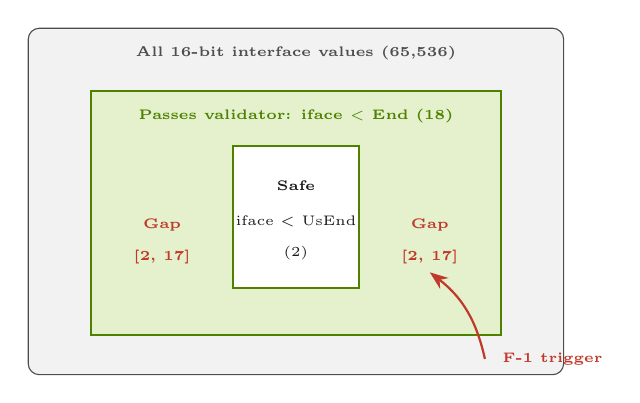
\begin{tikzpicture}[scale=1.0,every node/.style={transform shape}]
        % Universe of inputs
        \draw[rounded corners,fill=nvlight,draw=nvgray]
          (-3.4,-2.0) rectangle (3.4,2.4);
        \node[font=\tiny\bfseries,nvgray,anchor=north] at (0,2.3)
          {All 16-bit interface values (65{,}536)};

        % Validated region
        \draw[fill=nvgreen!20,draw=nvgreendark,thick]
          (-2.6,-1.5) rectangle (2.6,1.6);
        \node[font=\tiny\bfseries,nvgreendark,anchor=north] at (0,1.5)
          {Passes validator: iface $<$ End (18)};

        % Safe region
        \draw[fill=white,draw=nvgreendark,thick]
          (-0.8,-0.9) rectangle (0.8,0.9);
        \node[font=\tiny\bfseries,nvblack,align=center] at (0,0.4)
          {Safe};
        \node[font=\tiny,nvblack,align=center] at (0,-0.05)
          {iface $<$ UsEnd};
        \node[font=\tiny,nvblack,align=center] at (0,-0.45)
          {(2)};

        % Bug zone label - inside the green band but outside white
        \node[font=\tiny\bfseries,nvred] at (-1.7,-0.1) {Gap};
        \node[font=\tiny\bfseries,nvred] at (-1.7,-0.5) {[2, 17]};
        \node[font=\tiny\bfseries,nvred] at ( 1.7,-0.1) {Gap};
        \node[font=\tiny\bfseries,nvred] at ( 1.7,-0.5) {[2, 17]};

        % Arrow
        \draw[->,thick,nvred,>=Stealth] (2.4,-1.8)
          to[bend right=20] (1.7,-0.7);
        \node[font=\tiny\bfseries,nvred,align=center,anchor=west]
          at (2.5,-1.8) {F-1 trigger};
      \end{tikzpicture}

      \vspace{0.3em}
      {\scriptsize ESBMC explores \hil{the entire green zone} symbolically;
      fuzzing samples a handful of points.}
    \end{column}
  \end{columns}
\end{frame}

%% =================================================================
\begin{frame}{What is formal verification, in engineering terms?}
  \begin{block}{The idea}
    \small
    Translate the source code and a property (``no out-of-bounds access'',
    ``no overflow'', ``output is in $[0, 100]$'') into \hil{logical equations}.
    Hand them to a solver. The solver either \hil{proves the property holds
    for every input}, or returns a \hil{concrete counterexample} that breaks it.
  \end{block}

  \vspace{0.2em}
  \begin{columns}[T,onlytextwidth]
    \begin{column}{0.5\textwidth}
      \footnotesize
      \textbf{Three outcomes:}
      \begin{itemize}\setlength\itemsep{0.15em}
        \item \textcolor{nvgreendark}{\bfseries SAFE} — proven correct under
              the modelled bound.
        \item \textcolor{nvred}{\bfseries FAILED} — counterexample produced
              (concrete input + trace + failing assertion).
        \item \textcolor{nvgray}{\bfseries UNKNOWN} — solver gave up
              (rare for firmware-sized code).
      \end{itemize}
    \end{column}
    \begin{column}{0.5\textwidth}
      \footnotesize
      \textbf{Properties checked by default:}
      \begin{itemize}\setlength\itemsep{0.1em}
        \item Buffer / array out-of-bounds
        \item Null and dangling pointer dereferences
        \item Integer over- / underflow, div-by-zero
        \item Memory leaks, use-after-free
        \item Undefined-behaviour shifts, signed wraps
        \item Loop exhaustion — every loop is \hil{proven} to
              terminate within its stated bound (not silently truncated)
        \item \emph{User-defined} functional contracts
      \end{itemize}
    \end{column}
  \end{columns}

  \vspace{0.3em}
  {\scriptsize A counterexample is not a guess — it's a \hil{concrete input}
  the engineer can paste into a debugger and reproduce.}
\end{frame}

%% =================================================================
\begin{frame}[fragile]{How ESBMC proved F-1 — in three states}
  \begin{columns}[T,onlytextwidth]
    \begin{column}{0.46\textwidth}
      \footnotesize
      \textbf{Setup}
      \begin{itemize}\setlength\itemsep{0.1em}
        \scriptsize
        \item Harness constructs a Control SetEpId Request; 9 header
              fields constrained to pass \texttt{Validator::validate()}.
        \item \texttt{iface\_val} left \emph{nondeterministic} in $[2, 18)$.
        \item Calls production \texttt{on\_set\_endpoint\_id()} unmodified.
      \end{itemize}

      \vspace{0.3em}
      \textbf{Solver result}
      \begin{itemize}\setlength\itemsep{0.1em}
        \scriptsize
        \item 275 verification conditions generated.
        \item Bitwuzla returns SAT in \hil{$<$ 0.01 s}.
      \end{itemize}

      \vspace{0.3em}
      \textbf{Production confirmation}
      \begin{itemize}\setlength\itemsep{0.1em}
        \scriptsize
        \item Generated test case compiled and run natively.
        \item Process exits with \hil{SIGABRT (signal 6)}.
      \end{itemize}
    \end{column}

    \begin{column}{0.52\textwidth}
\begin{lstlisting}[basicstyle=\ttfamily\tiny,language={}]
ESBMC counterexample (abridged):

  State 5   iface_val = 2
            (passes assume >= UsEnd && < End)

  State 9   valid = 1
            (Validator::validate() returns true)

  State 10  Violated property:
            std::array::at out of range
            [i::0 < 2 fails]
            at set_cur_eid()
            -> cur_eid.at(2) on size-2 array

VERIFICATION FAILED
\end{lstlisting}

      \vspace{0.2em}
      {\scriptsize End-to-end proof from validator entry through dispatch
      to OOB write. \hil{No code modification, no manual test input.}}
    \end{column}
  \end{columns}
\end{frame}

%% =================================================================
\begin{frame}{Formal verification vs.\ traditional testing}
  \centering
  \renewcommand{\arraystretch}{1.05}
  \footnotesize
  \begin{tabular}{@{} p{0.27\textwidth} p{0.32\textwidth} p{0.32\textwidth} @{}}
    \toprule
    & \textbf{Traditional testing} & \textbf{Formal verification} \\
    \midrule
    Coverage of input space
      & A finite, hand-picked sample (or random for fuzz)
      & \hil{Symbolic — every input in the modelled range} \\
    Bug discovery
      & Finds bugs you anticipated
      & \hil{Finds bugs no one thought to test} \\
    Bug evidence
      & Failing test + stack trace
      & \hil{Auto-generated input + full executable trace} \\
    Concurrency
      & Schedule-dependent — bug only on rare interleavings
      & \hil{Explores all thread interleavings symbolically} \\
    Cost per defect (late)
      & High — found in QA / field
      & \hil{Low — found pre-commit} \\
    Maintenance
      & Tests rot; coverage drifts
      & Properties live next to the code; CI re-proves on every PR \\
    Confidence claim
      & ``We tested it''
      & \hil{``It cannot reach this state for any input''} \\
    Where it fails
      & Sparse coverage of the rare path
      & \hil{Large heap-aliasing problems;} known-finite loops are
        proven exhausted via unwinding assertions \\
    \bottomrule
  \end{tabular}

  \vspace{0.4em}
  \scriptsize
  \textit{The two are complementary, not competing. FV is most valuable on
  \hil{security-critical, hard-to-test, deeply-conditional} code paths —
  exactly the firmware control plane.}
\end{frame}

%% =================================================================
\begin{frame}{LLMs vs.\ formal verification --- complement, not replacement}
  \begin{columns}[T,onlytextwidth]
    \begin{column}{0.5\textwidth}
      \footnotesize
      \textbf{Where LLMs win (and where they break)}
      \begin{itemize}\setlength\itemsep{0.1em}
        \item Strong on \hil{small (20--100 LOC) snippets}; broad CWE
              coverage incl.\ non-formal classes (SQL injection,
              weak crypto, hard-coded credentials).
        \item Honest data: GPT-o3-mini scores \hil{955} on CASTLE
              vs.\ ESBMC \hil{697} on the same 250 micro-benchmarks
              (TASE 2025).
        \item \bad{But} on a 400+ LOC merged file LLMs
              \bad{hallucinate} false positives and \bad{miss hidden
              vulnerabilities}.
        \item \bad{Non-deterministic}: same prompt $\to$ different
              answers. No counterexample. No proof. No CI gate.
      \end{itemize}
    \end{column}

    \begin{column}{0.5\textwidth}
      \footnotesize
      \textbf{Where ESBMC wins (the firmware case)}
      \begin{itemize}\setlength\itemsep{0.1em}
        \item Every alarm ships with an \hil{executable
              counterexample} --- auditable, replayable, deterministic.
        \item FP rate is \hil{structurally bounded}: a counterexample
              either reproduces or it does not.
        \item Scales to \hil{whole-TU memory-safety properties}; F-1
              was found this way in sub-second proofs.
        \item Re-runs \hil{identically on every PR} --- a real CI gate.
      \end{itemize}
    \end{column}
  \end{columns}

  \vspace{0.5em}
  \begin{block}{Integration message}
    \scriptsize
    \hil{LLM in the IDE} for breadth and real-time hints.
    \hil{ESBMC at the CI gate} for memory-safety guarantees on firmware
    control paths. CASTLE's best two-tool combo is FV + classical SAST
    (\hil{ESBMC + CodeQL = 831}), with LLMs feeding the developer loop
    upstream --- not gating the merge.
  \end{block}
\end{frame}

%% =================================================================
\begin{frame}{The OpenSMA pilot at a glance}
  \begin{columns}[T,onlytextwidth]
    \begin{column}{0.52\textwidth}
      {\footnotesize\textbf{Scope (1 engineer, 9 days: 25 Apr -- 3 May 2026)}}
      \begin{itemize}\setlength\itemsep{0.05em}
        \scriptsize
        \item \hil{22 firmware modules}, $\sim$\hil{7{,}900 LOC} —
              roughly \hil{7\%} of the first-party C++ in OpenSMA.
        \item Targeted the MCTP/NSM control plane, I2C sensor drivers,
              and security-relevant validators; skipped vendored
              \texttt{libspdm} ($\sim$280\,k LOC) and FreeRTOS / MCU SDK
              glue ($\sim$45\,k LOC).
        \item Three phases: language-level safety (with loop-exhaustion
              assertions), $k$-induction over functional contracts, and
              a separate volatile-check phase --- plus negative tests
              that produce the F-* counterexamples. All proofs
              \hil{sub-second}.
      \end{itemize}

      \vspace{0.3em}
      {\footnotesize\textbf{Findings (8 active, 3 retracted)}}
      \begin{itemize}\setlength\itemsep{0.05em}
        \tiny
        \item \bad{Confirmed reachable (3):}
              \bad{F-1} abort path in MCTP dispatch
              (\href{https://github.com/NVIDIA/OpenSMA/issues/1}{\hil{NVIDIA/OpenSMA\#1}});
              F-6 unchecked \texttt{mode} byte stored in error-injection
              config; F-7 dirty \texttt{portRecoveryResp} written before
              validation.
        \item Latent today (5):
              F-4 UB shift in \texttt{operator""\_bit};
              F-5 missing bounds guard in \texttt{set\_bit} on the
              8-byte event bitmask;
              F-8 fixed-index \texttt{gpio\_ei\_entries[16]} OOB;
              F-10 silent 125\,\textdegree{}C substitution in busbar
              threshold setter (dead code: \texttt{BusBarTempSensorNum\,=\,0}
              on all current platforms);
              F-13 negative-percent wrap in debug-telemetry SMA
              (system proof shows upstream \texttt{std::clamp} blocks it).
        \item \hil{Retracted on review:} F-2, F-3, F-14.
      \end{itemize}
    \end{column}

    \hfill
    \begin{column}{0.46\textwidth}
      \begin{block}{Modules covered}
        \tiny
        MCTP packet parser \textbar{} MCTP routing helpers \textbar{}
        MCTP dispatch \textbar{} MCTP validator state machine \textbar{}
        Fixed-point arithmetic \textbar{} Saturating arithmetic \textbar{}
        NSM type-2 PCIe-link reset \textbar{} NSM type-3 sensor availability
        \textbar{} NSM type-5 field validators \textbar{} NSM event bitmask
        \textbar{} Telemetry sensor-ID lookup \textbar{} SPI byte-buffer
        (de)serialisation \textbar{} I2C CRC-8 \textbar{} User-defined
        integer literals \textbar{} NTC thermistor table \textbar{}
        Power-smoothing presets \textbar{} FRU utilities \textbar{}
        SoC SMA filter \textbar{} Debug-telemetry SMA \textbar{}
        PCA9555 GPIO expander \textbar{} EMC1812 temp sensor \textbar{}
        TMP1075 temp sensor \textbar{} TMP461 temp sensor
      \end{block}

      \begin{block}{Verification budget}
        \scriptsize
        $\sim$5{,}000 verification conditions across Phase~1, Phase~2
        ($k$-induction), volatile-check, and negative tests --- all solved
        sub-second on Bitwuzla 0.8.2. Reproducible with \texttt{make all}.
      \end{block}
    \end{column}
  \end{columns}
\end{frame}

%% =================================================================
\begin{frame}{Tangible value: ROI for firmware}
  \begin{columns}[T,onlytextwidth]
    \begin{column}{0.5\textwidth}
      \footnotesize
      \textbf{Direct savings}
      \begin{itemize}\setlength\itemsep{0.1em}
        \item One F-1-class issue caught \hil{pre-ship} avoids field
              debug, OTA / RMA cost, disclosure / CVE handling, brand impact.
        \item Industry benchmark: a defect found post-release costs
              \hil{30--100$\times$} a defect found in requirements /
              early design.
      \end{itemize}

      \vspace{0.3em}
      \textbf{Speed of iteration}
      \begin{itemize}\setlength\itemsep{0.1em}
        \item Sub-second proofs $\Rightarrow$ PR CI with
              \hil{linter-class latency}.
        \item Unlike a linter, the verdict is a \hil{mathematical proof
              over all inputs}, not a pattern match.
        \item CASTLE (TASE 2025): ESBMC tops 13 SAST tools on 250 CWE
              programs --- \hil{12 false positives vs.\ 259--1{,}104}.
      \end{itemize}
    \end{column}

    \begin{column}{0.5\textwidth}
      \footnotesize
      \textbf{Compounding value}
      \begin{itemize}\setlength\itemsep{0.1em}
        \item Properties written once; \hil{re-proven on every commit, forever}
              --- linters only know rules their authors shipped.
        \item Catches regressions as the code evolves —
              testing's biggest blind spot.
        \item Property files double as
              \hil{executable specifications} for new engineers.
      \end{itemize}

      \vspace{0.3em}
      \textbf{Safety \& certification leverage}
      \begin{itemize}\setlength\itemsep{0.1em}
        \item Counts toward \hil{ISO 26262 / IEC 61508} unit-level evidence.
        \item Required or recommended in DO-178C (avionics),
              EN 50128 (rail), and emerging automotive ASIL-D expectations.
      \end{itemize}
    \end{column}
  \end{columns}

  \vspace{0.3em}
  {\tiny\textcolor{nvgray}{Cost ratio: Boehm, \emph{Software Engineering
  Economics} (Prentice-Hall, 1981), Fig.\ 4-2, p.\ 40; RTI, \emph{The
  Economic Impacts of Inadequate Infrastructure for Software Testing},
  NIST Planning Report 02-3 (2002), Tables 1-1 and 5-2. F-1 contains
  no anti-pattern targeted by clang-tidy / cppcheck / MISRA-C 2012.}}
\end{frame}

%% =================================================================
\begin{frame}{Risk reduction \& strategic differentiation}
  \begin{columns}[T,onlytextwidth]
    \begin{column}{0.5\textwidth}
      \footnotesize
      \textbf{Bug classes formal verification eliminates}
      \begin{itemize}\setlength\itemsep{0.1em}
        \item Memory-safety violations (OOB, UAF, null deref).
        \item Integer over- / underflow on critical paths.
        \item Concurrency races --- bugs hidden in one interleaving
              out of millions; tests almost never reproduce them.
        \item Protocol-state-machine violations.
        \item Implicit standard-conformance issues (shift UB, etc.).
      \end{itemize}

      \vspace{0.3em}
      \textbf{These are the bug classes that drive}
      \begin{itemize}\setlength\itemsep{0.1em}
        \item firmware-borne CVEs,
        \item silent data corruption,
        \item watchdog-induced reboots in the field.
      \end{itemize}
    \end{column}

    \begin{column}{0.5\textwidth}
      \footnotesize
      \textbf{Differentiation for NVIDIA}
      \begin{itemize}\setlength\itemsep{0.15em}
        \item Datacenter customers increasingly ask for
              \hil{provable} security properties on management firmware.
        \item Hyperscaler procurement teams already require formal
              evidence for boot / attestation paths.
        \item ``\hil{Verified} by formal methods'' is a credible
              market message — not marketing language.
        \item Public examples of FV on critical firmware include
              AWS (s2n), Microsoft (Azure RTOS),
              Google (Android Verified Boot, Titan-M),
              Apple (sepOS), and Arm (CCA).
      \end{itemize}
    \end{column}
  \end{columns}
\end{frame}

%% =================================================================
\begin{frame}{Where formal verification fits in the firmware workflow}
  \centering
  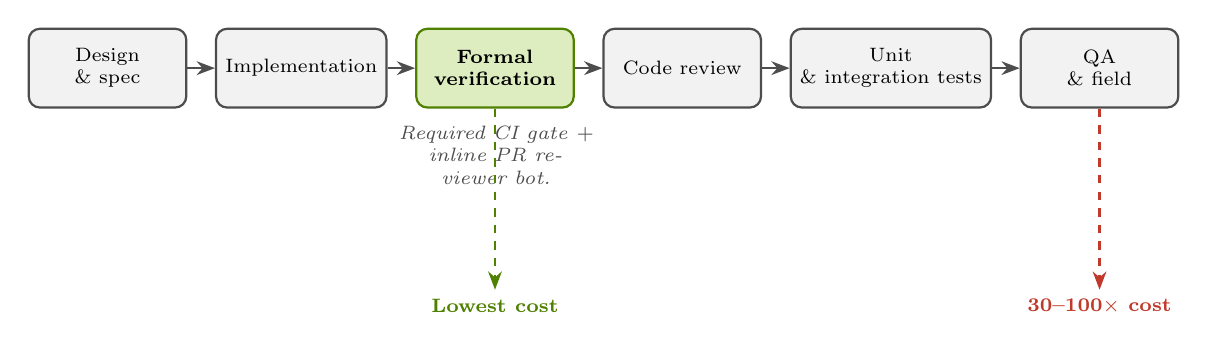
\begin{tikzpicture}[
    node distance=0.4cm and 0.35cm,
    box/.style={rectangle,rounded corners,draw=nvgray,thick,
                minimum height=1.0cm,minimum width=2.0cm,align=center,
                font=\scriptsize,fill=nvlight},
    fvbox/.style={box,fill=nvgreen!25,draw=nvgreendark,thick,
                  font=\scriptsize\bfseries},
    arr/.style={->,>=Stealth,thick,nvgray},
    label/.style={font=\scriptsize\itshape,nvgray}
  ]
    \node[box] (design)  {Design \\ \& spec};
    \node[box,right=of design] (code) {Implementation};
    \node[fvbox,right=of code] (fv) {Formal\\verification};
    \node[box,right=of fv] (review) {Code review};
    \node[box,right=of review] (test) {Unit \\ \& integration tests};
    \node[box,right=of test] (qa) {QA \\ \& field};

    \draw[arr] (design) -- (code);
    \draw[arr] (code) -- (fv);
    \draw[arr] (fv) -- (review);
    \draw[arr] (review) -- (test);
    \draw[arr] (test) -- (qa);

    \node[label,below=0.1cm of fv,text width=2.6cm,align=center]
      (fvnote) {Required CI gate \emph{+}\\inline PR reviewer bot.};

    % Cost callouts on a single baseline below the row
    \node[font=\scriptsize\bfseries,nvgreendark,below=2.3cm of fv]
      (fvcost) {Lowest cost};
    \draw[->,>=Stealth,thick,nvgreendark,dashed] (fv.south) -- (fvcost.north);

    \node[font=\scriptsize\bfseries,nvred,below=2.3cm of qa]
      (qacost) {30--100$\times$ cost};
    \draw[->,>=Stealth,thick,nvred,dashed] (qa.south) -- (qacost.north);
  \end{tikzpicture}

  \vspace{0.4em}
  \footnotesize
  Formal verification slots in \hil{between implementation and review},
  catching defects when fixing them is cheapest. ESBMC runs as a
  \hil{required CI check} \emph{and} posts each counter-example as an
  inline PR review comment --- a CodeRabbit-style bot, but with
  \hil{proofs in place of heuristics}: every comment carries a
  \hil{concrete reproducer}, not a hunch. Counterexamples become
  regression tests automatically --- feeding the existing test pyramid.

  \vspace{0.3em}
  {\tiny\textcolor{nvgray}{Cost ratio: Boehm, \emph{Software Engineering
  Economics} (Prentice-Hall, 1981), Fig.\ 4-2, p.\ 40; RTI, \emph{The
  Economic Impacts of Inadequate Infrastructure for Software Testing},
  NIST Planning Report 02-3 (2002), Tables 1-1 and 5-2.}}
\end{frame}

%% =================================================================
\begin{frame}{Tooling investment \& ecosystem position}
  \begin{columns}[T,onlytextwidth]
    \begin{column}{0.5\textwidth}
      \footnotesize
      \textbf{What was used}
      \begin{itemize}\setlength\itemsep{0.1em}
        \item \hil{ESBMC 8.2} — open source, actively maintained by
              the SSV Lab (Univ.\ of Manchester / Federal Univ.\ of
              Amazonas), with contributors from Southampton and
              Stellenbosch.
        \item \hil{Bitwuzla} SMT solver — state-of-the-art on
              bitvector / array theories.
        \item Tool footprint: a single binary + the existing build system.
      \end{itemize}

      \vspace{0.3em}
      \textbf{What was contributed back}
      \begin{itemize}\setlength\itemsep{0.1em}
        \item \hil{20+ ESBMC bug reports / fixes} filed during the
              pilot — most merged upstream.
        \item Hardens the tool for everyone using it on C++20
              firmware (including future NVIDIA work).
      \end{itemize}
    \end{column}

    \begin{column}{0.5\textwidth}
      \footnotesize
      \textbf{What this looks like at scale}
      \begin{itemize}\setlength\itemsep{0.1em}
        \item Property files live next to source headers.
        \item $\sim$1 hour per new module to set up.
        \item CI gate: PR fails if a property regresses.
        \item No license cost. No vendor lock-in.
      \end{itemize}

      \vspace{0.3em}
      \textbf{Pricing model: pay for services, not the tool}
      \begin{itemize}\setlength\itemsep{0.1em}
        \item \hil{Foundation:} priority bug-fix queue + quarterly
              training --- low-commitment on-ramp.
        \item \hil{Per-module:} fixed-price end-to-end verification
              (harness, properties, CI, 12-mo maintenance).
        \item \hil{Partnership retainer:} embedded engineers, PR-bot
              / certification kits, ESBMC roadmap influence.
        \item Tool stays \hil{open source --- no licence, no lock-in};
              fits NVIDIA's academic-research sponsorship pattern.
      \end{itemize}
    \end{column}
  \end{columns}
\end{frame}

%% =================================================================
\begin{frame}{Recommendation}
  \begin{block}{Three concrete next steps}
    \begin{enumerate}
      \item \hil{Land the eight finding fixes.}
            F-1, F-6, F-7 reachable; F-4, F-5, F-8, F-10, F-13 latent
            (one-line patches; harnesses in tree).
      \item \hil{Add the OpenSMA verification suite to CI.}
            \texttt{make all} runs in seconds; gate every PR on it.
            Catches the next F-1 the day it's introduced.
      \item \hil{Pick one new NVIDIA firmware module to verify next quarter.}
            Choose a security-critical surface (boot, attestation, key
            management, MCTP / NSM dispatch elsewhere). Re-evaluate ROI
            with internal numbers in 90 days.
    \end{enumerate}
  \end{block}

  \vspace{0.4em}
  \begin{columns}[T,onlytextwidth]
    \begin{column}{0.5\textwidth}
      \textbf{What we are asking for}
      \begin{itemize}
        \footnotesize
        \item Engineering sponsorship to merge fixes \& enable CI.
        \item One firmware module per quarter as a verification target.
        \item A 90-day check-in to review hit rate vs.\ effort.
      \end{itemize}
    \end{column}
    \begin{column}{0.5\textwidth}
      \textbf{What it costs}
      \begin{itemize}
        \footnotesize
        \item Open-source tooling: \$0.
        \item CI compute: negligible (sub-second proofs).
        \item Engineering effort: $\sim$0.5 FTE to scale to a
              second module + maintain CI.
      \end{itemize}
    \end{column}
  \end{columns}
\end{frame}

%% =================================================================
\begin{frame}{Summary in three lines}
  \vspace{1.2em}
  \begin{block}{}
    \large
    \begin{enumerate}
      \item Formal verification \hil{produced a counterexample for a real
            abort path} in OpenSMA that manual review and unit testing
            had missed (filed upstream for triage).
      \item It did so in \hil{seconds}, on a laptop, with \hil{open-source
            tooling} and \hil{no production code changes}.
      \item Adopting it as a CI gate is a \hil{low-cost, high-leverage}
            way to harden NVIDIA firmware against a whole class of
            field-stopping defects.
    \end{enumerate}
  \end{block}

  \vspace{1.0em}
  \centering
  \large \textcolor{nvgreendark}{\textbf{Thank you.}} \\
  \vspace{0.4em}
  \footnotesize
  Full report: \texttt{verification/REPORT.md} \\
  Reproduce: \texttt{cd verification \&\& make all}

  \vspace{0.8em}
  {\tiny\textcolor{nvgray}{Independent research, University of Manchester.
  NVIDIA, OpenSMA, and related marks are trademarks of NVIDIA Corporation;
  no affiliation or endorsement implied.}}
\end{frame}

%% =================================================================
%% Backup
%% =================================================================
\appendix

\begin{frame}{Backup --- The validator gap, in numbers}
  \footnotesize
  \begin{tabular}{@{} l l l @{}}
    \toprule
    \textbf{Symbol} & \textbf{Value} & \textbf{Where defined} \\
    \midrule
    \texttt{Interface::UsEnd}   & 2  & \texttt{Packet.h} (size of \texttt{cur\_eid} array) \\
    \texttt{Interface::End}     & 18 & \texttt{Packet.h} (validator's upper bound) \\
    Gap range                   & $[2, 17]$ & 16 values that pass validation but OOB the array \\
    \texttt{InterfaceType} type & \texttt{uint16\_t} & full domain $2^{16}$ values \\
    \bottomrule
  \end{tabular}

  \vspace{0.6em}
  \textbf{Two equally good fixes:}
  \begin{itemize}
    \item Add \texttt{if (interface >= UsEnd) return;} to \texttt{set\_cur\_eid()}
          — match the guard that \texttt{get\_cur\_eid()} already carries.
    \item Tighten \texttt{Validator::validate()} to reject
          \texttt{interface >= UsEnd} instead of \texttt{>= End} — closes the gap
          at the validator boundary.
  \end{itemize}
\end{frame}

\begin{frame}{Backup --- Why ESBMC, specifically}
  \footnotesize
  \begin{itemize}
    \item \hil{Open source.} No license barrier to internal
          adoption or experimentation.
    \item \hil{C++20-aware}, with active maintenance — most defects we
          encountered during the pilot were fixed upstream within days.
    \item Uses industrial-strength SMT solvers
          (\hil{Bitwuzla}, \hil{Z3}). No bespoke proof language.
    \item \hil{Counterexample-first} workflow: failing properties produce
          concrete inputs that engineers can reproduce immediately.
    \item Generates \hil{CTest-compatible test cases} — counterexamples
          become regression tests automatically.
    \item \hil{k-induction} support for proving loop / state-machine
          invariants without unbounded unrolling.
    \item Backed by 15+ years of academic research and supported by
          \hil{ARM, AWS, Intel, Samsung, Motorola Mobility, Nokia Institute of
          Technology}, the Ethereum and Rust Foundations, EPSRC, UKRI, EU
          Horizon 2020, and Brazilian agencies CNPq / CAPES / FAPEAM.
  \end{itemize}
\end{frame}

\begin{frame}{Backup --- ESBMC vs.\ static analysis: independent benchmark}
  \scriptsize
  \textbf{CASTLE} (TASE 2025): 250 C programs, 25 CWEs; 13 static
  analysers, 2 formal verifiers, 10 LLMs evaluated head-to-head.

  \vspace{0.3em}
  \centering
  \renewcommand{\arraystretch}{0.95}
  \begin{tabular}{@{} l r r r r r @{}}
    \toprule
    \textbf{Tool} & \textbf{TP} & \textbf{FP} & \textbf{P}
                  & \textbf{R} & \textbf{CASTLE} \\
    \midrule
    \hil{ESBMC} (FV)        & 53  & \hil{12}    & 82\% & 35\% & \hil{697} \\
    CodeQL                  & 35  & 43          & 45\% & 23\% & 600 \\
    Cppcheck                & 18  & 5           & 78\% & 12\% & 405 \\
    Clang Analyzer          & 13  & 2           & 87\% &  9\% & 381 \\
    Splint                  & 23  & 1{,}029     &  2\% & 15\% & $-600$ \\
    CodeThreat              & 21  & 1{,}104     &  2\% & 14\% & $-710$ \\
    \midrule
    \hil{GPT-o3-mini} (LLM) & 121 & 72          & 63\% & 81\% & \hil{955} \\
    DeepSeek R1 (LLM)       & 133 & 163         & 45\% & 89\% & 888 \\
    GPT-4o (LLM)            & 113 & 141         & 44\% & 75\% & 814 \\
    LLAMA 3.1 8B (LLM)      & 56  & 374         & 13\% & 37\% & 245 \\
    \bottomrule
  \end{tabular}

  \vspace{0.2em}
  \raggedright
  \begin{itemize}\setlength\itemsep{0.02em}
    \item \hil{Top reasoning LLMs beat all SAST + FV tools} on 20--100
          LOC snippets --- but accuracy \bad{collapses past $\sim$400
          LOC} and is \bad{non-deterministic}; ESBMC's 12 FPs come with
          reproducible counterexamples.
    \item ESBMC is the \hil{highest-scoring non-LLM tool}; best
          two-tool combo is \hil{ESBMC + CodeQL = 831}
          ($+134$ over ESBMC alone) --- complementary, not competing.
    \item SAST tools split into high-precision / low-recall (Cppcheck,
          Clang) or runaway-FP (Splint, CodeThreat).
  \end{itemize}

  \vspace{0.1em}
  {\tiny\textcolor{nvgray}{Dubniczky et al., \emph{CASTLE: Benchmarking
  Dataset for Static Code Analyzers and LLMs towards CWE Detection},
  TASE 2025, Table 3. Dataset:~\texttt{github.com/CASTLE-Benchmark}.}}
\end{frame}

\end{document}
